\let\negmedspace\undefined
\let\negthickspace\undefined
\documentclass[journal]{IEEEtran}
\usepackage[a5paper, margin=10mm, onecolumn]{geometry}
%\usepackage{lmodern} % Ensure lmodern is loaded for pdflatex
\usepackage{tfrupee} % Include tfrupee package

\setlength{\headheight}{1cm} % Set the height of the header box
\setlength{\headsep}{0mm}     % Set the distance between the header box and the top of the text

\usepackage{gvv-book}
\usepackage{gvv}
\usepackage{cite}
\usepackage{amsmath,amssymb,amsfonts,amsthm}
\usepackage{algorithmic}
\usepackage{graphicx}
\usepackage{textcomp}
\usepackage{xcolor}
\usepackage{txfonts}
\usepackage{listings}
\usepackage{enumitem}
\usepackage{mathtools}
\usepackage{gensymb}
\usepackage{comment}
\usepackage[breaklinks=true]{hyperref}
\usepackage{tkz-euclide} 
\usepackage{listings}
% \usepackage{gvv}                                        
\def\inputGnumericTable{}                                 
\usepackage[latin1]{inputenc}                                
\usepackage{color}                                            
\usepackage{array}                                            
\usepackage{longtable}                                       
\usepackage{calc}                                             
\usepackage{multirow}                                         
\usepackage{hhline}                                           
\usepackage{ifthen}                                           
\usepackage{lscape}
\usepackage{circuitikz}
\tikzstyle{block} = [rectangle, draw, fill=blue!20, 
    text width=4em, text centered, rounded corners, minimum height=3em]
\tikzstyle{sum} = [draw, fill=blue!10, circle, minimum size=1cm, node distance=1.5cm]
\tikzstyle{input} = [coordinate]
\tikzstyle{output} = [coordinate]


\begin{document}

\bibliographystyle{IEEEtran}
\vspace{3cm}

\title{4.13.31}
\author{EE25BTECH11026-Harsha}
 \maketitle
% \newpage
% \bigskip
{\let\newpage\relax\maketitle}

\renewcommand{\thefigure}{\theenumi}
\renewcommand{\thetable}{\theenumi}
\setlength{\intextsep}{10pt} % Space between text and floats


\numberwithin{equation}{enumi}
\numberwithin{figure}{enumi}
\renewcommand{\thetable}{\theenumi}

\textbf{Question}:\\
Line L has intercepts a and b on the coordinate axes. When the axes are rotated
through a given angle, keeping the origin fixed, line L has intercepts p and q. Then
\begin{multicols}{4}
\begin{enumerate}
    \item $a^2+b^2=p^2+q^2$
    \item $\frac{1}{a^2}+\frac{1}{b^2}=\frac{1}{p^2}+\frac{1}{q^2}$
    \item $a^2+p^2=b^2+q^2$
    \item $\frac{1}{a^2}+\frac{1}{p^2}=\frac{1}{b^2}+\frac{1}{q^2}$
\end{enumerate}
\end{multicols}
\solution \\
Let us solve the given question theoretically and then verify the solution computationally.\\
\\
According to the question,\\
\begin{align}
    \text{The equation of line\,:\,}\myvec{\frac{1}{a}&&\frac{1}{b}}\vec{x}=1
\end{align} 
Let the row coefficient vector of the original line be $\vec{m}$ and for the rotated line be $\vec{m'}$.

\begin{align}
     \vec{m'}=\vec{P}\vec{m}       
\end{align}
where $\vec{P}$ is the rotation matrix
\begin{align}
    \|\vec{m'}\|^2=\vec{m'}^{\top}\vec{m'}=\brak{\vec{m}^{\top}\vec{P}^{\top}}\brak{\vec{P}\vec{m}}=\vec{m}^{\top}\brak{\vec{P}^{\top}\vec{P}}\vec{m}
\end{align}
Since $\vec{P}$ is an orthogonal matrix,
\begin{align}
    \therefore \vec{m}^{\top}\brak{\vec{P}^{\top}\vec{P}}\vec{m}=\vec{m}^{\top}\vec{m}=\|m\|^2
\end{align}
\begin{align}
    \implies \|\vec{m'}\|^2=\|\vec{m}\|^2
\end{align}
As $\vec{m'}$ is given by $\myvec{\frac{1}{p}&&\frac{1}{q}}^{\top}$,
\begin{align}
    \therefore \frac{1}{p^2}+\frac{1}{q^2}=\frac{1}{a^2}+\frac{1}{b^2}
\end{align}

\newpage
\vspace*{0.25cm}

From the figure, it is clearly verified that the theoretical solution matches with the computational solution.\\
\begin{figure}[H]
    \centering
    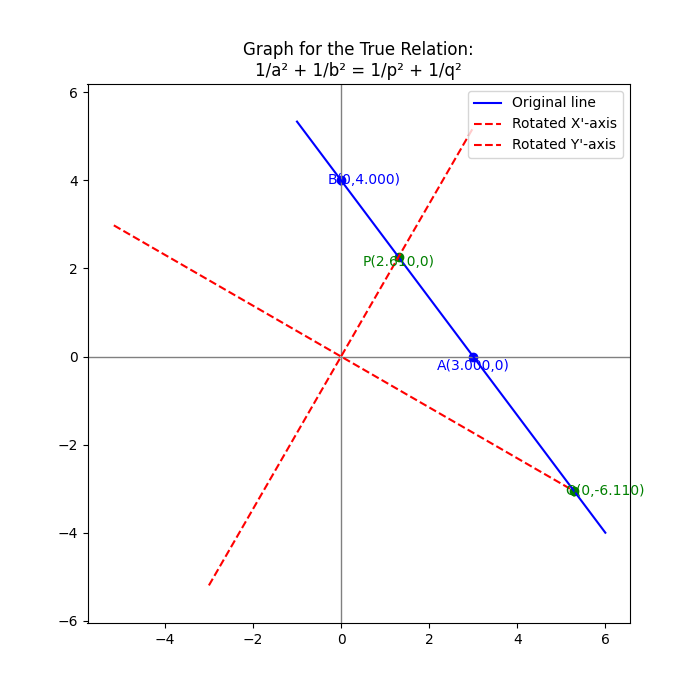
\includegraphics[width=0.8\columnwidth]{figs/Figure_1.png}
    \label{fig:1}
\end{figure}

\end{document}
